\documentclass[12pt,fleqn]{article}\usepackage{../../common}
\begin{document}

\begin{minted}[fontsize=\footnotesize]{python}
import pandas as pd, zipfile
import numpy as np
import cv2

def draw_flow(img, flow, step=16):
    h, w = img.shape[:2]
    y, x = np.mgrid[step/2:h:step, step/2:w:step].reshape(2,-1).astype(int)
    fx, fy = flow[y,x].T
    lines = np.vstack([x, y, x+fx, y+fy]).T.reshape(-1, 2, 2)
    lines = np.int32(lines + 0.5)
    vis = cv2.cvtColor(img, cv2.COLOR_GRAY2BGR)
    cv2.polylines(vis, lines, 0, (0, 255, 0))
    for (x1, y1), (x2, y2) in lines:
        cv2.circle(vis, (x1, y1), 1, (0, 255, 0), -1)
    return vis

prevgray = cv2.imread('106.jpg', cv2.IMREAD_GRAYSCALE)
gray = cv2.imread('107.jpg', cv2.IMREAD_GRAYSCALE)
flow = cv2.calcOpticalFlowFarneback(prevgray, gray, None, 0.5, 3, 15, 3, 5, 1.2, 0)
cv2.imwrite('vision_30vstab_01.png', draw_flow(gray, flow))
\end{minted}


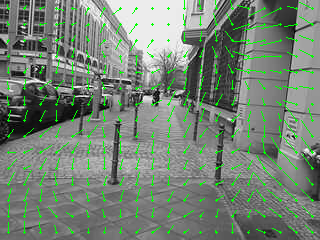
\includegraphics[width=20em]{vision_30vstab_01.png}












\end{document}
